%	This is written by Zhiyang Ong as a template for writing reports.

%	The MIT License (MIT)

%	Copyright (c) <2014> <Zhiyang Ong>

%	Permission is hereby granted, free of charge, to any person obtaining a copy of this software and associated documentation files (the "Software"), to deal in the Software without restriction, including without limitation the rights to use, copy, modify, merge, publish, distribute, sublicense, and/or sell copies of the Software, and to permit persons to whom the Software is furnished to do so, subject to the following conditions:

%	The above copyright notice and this permission notice shall be included in all copies or substantial portions of the Software.

%	THE SOFTWARE IS PROVIDED "AS IS", WITHOUT WARRANTY OF ANY KIND, EXPRESS OR IMPLIED, INCLUDING BUT NOT LIMITED TO THE WARRANTIES OF MERCHANTABILITY, FITNESS FOR A PARTICULAR PURPOSE AND NONINFRINGEMENT. IN NO EVENT SHALL THE AUTHORS OR COPYRIGHT HOLDERS BE LIABLE FOR ANY CLAIM, DAMAGES OR OTHER LIABILITY, WHETHER IN AN ACTION OF CONTRACT, TORT OR OTHERWISE, ARISING FROM, OUT OF OR IN CONNECTION WITH THE SOFTWARE OR THE USE OR OTHER DEALINGS IN THE SOFTWARE.

%	Email address: echo "cukj -wb- 23wU4X5M589 TROJANS cqkH wiuz2y 0f Mw Stanford" | awk '{ sub("23wU4X5M589","F.d_c_b. ") sub("Stanford","d0mA1n"); print $5, $2, $8; for (i=1; i<=1; i++) print "6\b"; print $9, $7, $6 }' | sed y/kqcbuHwM62z/gnotrzadqmC/ | tr 'q' ' ' | tr -d [:cntrl:] | tr -d 'ir' | tr y "\n"

%%%%%%%%%%%%%%%%%%%%%%%%%%%%%%%%%%%%%%%%%%%%%%









%%%%%%%%%%%%%%%%%%%%%%%%%%%%%%%%%%%%%%%%%%%%%%
%	Preamble.
\documentclass[letterpaper,12pt]{report}
%%%%%%%%%%%%%%%%%%%%%%%%%%%%%%%%%%%%%%%%%%%%%
%
%	Importing LaTeX source files, without quoting the ".tex" extension.
%
%%%%%%%%%%%%%%%%%%%%%%%%%%%%%%%%%%%%%%%%%%%%%

%%%%%%%%%%%%%%%%%%%%%%%%%%%%%%%%%%%%%%%%%%%%%
%	File containing the LaTeX preamble.
% This is written by Zhiyang Ong as the preamble for all his LaTeX documents.
%
% It includes a list of LaTeX packages that he commonly uses to typeset LaTeX documents.

%	The MIT License (MIT)

%	Copyright (c) <2014> <Zhiyang Ong>

%	Permission is hereby granted, free of charge, to any person obtaining a copy of this software and associated documentation files (the "Software"), to deal in the Software without restriction, including without limitation the rights to use, copy, modify, merge, publish, distribute, sublicense, and/or sell copies of the Software, and to permit persons to whom the Software is furnished to do so, subject to the following conditions:

%	The above copyright notice and this permission notice shall be included in all copies or substantial portions of the Software.

%	THE SOFTWARE IS PROVIDED "AS IS", WITHOUT WARRANTY OF ANY KIND, EXPRESS OR IMPLIED, INCLUDING BUT NOT LIMITED TO THE WARRANTIES OF MERCHANTABILITY, FITNESS FOR A PARTICULAR PURPOSE AND NONINFRINGEMENT. IN NO EVENT SHALL THE AUTHORS OR COPYRIGHT HOLDERS BE LIABLE FOR ANY CLAIM, DAMAGES OR OTHER LIABILITY, WHETHER IN AN ACTION OF CONTRACT, TORT OR OTHERWISE, ARISING FROM, OUT OF OR IN CONNECTION WITH THE SOFTWARE OR THE USE OR OTHER DEALINGS IN THE SOFTWARE.

%	Email address: echo "cukj -wb- 23wU4X5M589 TROJANS cqkH wiuz2y 0f Mw Stanford" | awk '{ sub("23wU4X5M589","F.d_c_b. ") sub("Stanford","d0mA1n"); print $5, $2, $8; for (i=1; i<=1; i++) print "6\b"; print $9, $7, $6 }' | sed y/kqcbuHwM62z/gnotrzadqmC/ | tr 'q' ' ' | tr -d [:cntrl:] | tr -d 'ir' | tr y "\n"

%%%%%%%%%%%%%%%%%%%%%%%%%%%%%%%%%%%%%%%%%%%%%%%%%%

% Importing some standard LaTeX packages.

% To enable standard LaTeX processing for graphics. It enables PDF, JPEG, PNG, and TIFF graphics files to be included in the LaTeX document.
\usepackage{graphicx}
% For better typesetting of mathematical expressions, from the American Mathematical Society (AMS).
\usepackage{amsmath}
% For better typesetting of mathematical expressions, from the American Mathematical Society (AMS). This package includes mathematical symbols for the ``amsmath'' package.
\usepackage{amssymb}
% For better typesetting of mathematical proofs (for theorems and colloraries), from the American Mathematical Society (AMS).
\usepackage{amsthm}
%	Create definitions for new theorems, axioms, colloraries.
	\newtheorem{theorem}{Theorem}[chapter]
	\newtheorem{axiom}{Axiom}[chapter]
	\newtheorem{corollary}{Corollary}[chapter]
	\newtheorem{lemma}{Lemma}[chapter]
	\newtheorem{Rule}{Rule}[chapter]
	\newtheorem{law}{Law}[chapter]
	\newtheorem{principle}{Principle}[chapter]
% To change the style of newly defined theorems.
%		\usepackage{theorem}




%	Typesetting with the typewriter font.
%\usepackage{ttfamily}

% For better typesetting of tables (and arrays).
\usepackage{array}
% For creating tables without vertical separators.
%		\usepackage{booktabs}
% To control line spacing in LaTeX documents.
\usepackage{setspace}
% To modify the spacing between words and letters.
%		\usepackage{microtype}
% To change the dimensions of the page(s).
%\usepackage[margin=1.5cm,vmargin={0pt,1cm},nohead]{geometry}
\usepackage[margin=1.5cm,vmargin={1.5cm,2cm}]{geometry}
% Use the packages needed to typeset algorithms. I can also use the combined ``algorithms'' bundle.
\usepackage{algorithm}
\usepackage{algorithmic}
% The listings package is a source code printer for LaTeX. You can typeset stand alone files as well as listings with an environment similar to verbatim as well as you can print code snippets using a command similar to \verb. Many parameters control the output and if your preferred programming language isn�t already supported, you can make your own definition.
\usepackage{listings}
% Use the ``clrscode3e'' LaTeX package to typeset algorithms like CLRS
%	\usepackage{/data/others/notes/clrscode3e}
%/Applications/apps/comune/SienaLaTeX/rapporto/
\usepackage{/Applications/apps/comune/SienaLaTeX/rapporto/others/clrscode3e}
%\usepackage{/data/others/grappanotes/clrscode3e}
% Use the ``algpseudocode'' LaTeX package to typeset algorithms -- Alternate solution, not preferred
%\usepackage{algpseudocode}
% Alternative packages for typesetting algorithms.
%\usepackage{algorithm2e}
%\usepackage{algorithmicx}
%\usepackage{program}
%	To check for syntax errors in my LaTeX document.
\RequirePackage[l2tabu, orthodox]{nag}

% Concatenate adjacent references together when typeset.
% That is, cite{ref1,ref2,ref3,ref4} can appear as [12-15], instead of [12] [13] [14] [15]
\usepackage{cite}
% For automatic insertion of cross-referencing words, such as fig. for figures and eq. for equations.
%		\usepackage{cleveref}

% LaTeX support for Metafont and MetaPost logos.
\usepackage{mflogo}













% How to typeset single and double quotes for feet and inches?
% For feet, use [FEET]\textasciiacute
% For inches, use [INCHES]\textacutedbl
% For feet and inches, use [FEET]\textasciiacute\ [INCHES]\textacutedbl; force a character space between the single quote for feet and the height of the object in inches
% Don't use \textceltpal as a single quote to represent height in feet, or double \textceltpal (two concatenated \textceltpal) as a double quote to represent height in inches
% For double quotes, don't use two single quotes provided by the default settings of LaTeX. The resultant double quotes will be curly.

% The tipa package is for Phonetic Symbols -- I wanna use the \textceltpal symbol to represent a single quote, instead of using the generic ``curly'' single quote from \LaTeX (Table 10, pp.10)
\usepackage{tipa}
% The textcomp package is for Diacritics -- I wanna use the \textacutedbl symbol to represent a double quote (Table 28, pp.17), instead of using the generic ``curly'' double quotes from \LaTeX; however, when this symbol is used, I must force a character space to exist after the symbol by using the backslash followed by a character space. This package also provides the symbol for Copyleft, \textcopyleft, which is not available in LaTeX by default, and provides better looking symbols for: copyright, registered, and trademark (Table 33, pp.18). Also, it provides symbols for: \textcelsius, \textmho, \textmu, \textohm (Table 201, pp.67). It also provides symbols for Genealogical Symbols (Table 253, pp78), such as \textborn, \textdivorced, \textmarried, \textdied, and \textleaf (symbol of a leaf)... Its symbol for the Euro, EU currency, is \texteuro
\usepackage{textcomp}
% Look at \url{http://www.ctan.org/tex-archive/info/symbols/comprehensive/symbols-a4.pdf} for a list of symbols that can be used in LaTeX and its packages. Table 280, pp.88, deals with Symbol Name Clashes; hence, if the same command name refers to multiple symbols, the symbol-conflict resolution abides by this.
% In particular, check out the gensymb package (Table 197, page 67) for symbols defined to work in both math and text modes, such as \celsius, \micro, \degree, and \ohm.
% Also, check out the wasysym package (Table 198, page 67) for electrical symbols, such as that of alternating current (AC); it also provides symbols for \female, and \male (Table 212, pp.70); it also has symbols for ``Xs and Check Marks,'' which are checked boxes, \CheckedBox, squares, \Square, and crossed boxes (boxes filled with a cross), \XBox (Table 232, pp.73); it also has symbols for a clock, \clock, a Simley, \smiley, diameter, \diameter, lightning, \lightning, sun, \sun, and a tick or check mark \checked (symbol to indicate that something is correct), and a bell, \bell (Table 254, pp.78); it also has symbols for left and right turns (Table 256, pp.78), \leftturn and \rightturn; this package (Table 256, pp.78) and the arev package (Table 257, pp.78) can be used to typeset music symbols, along with Table 182, pp.62; it also has symbols for Navigation (Table 261, pp.79), such as \Forward, \RewindToStart, and \ForwardToIndex; it also has symbols for laundry (Table 262, pp.80); it also has the symbol for a heart, \Heart (Table 263, pp.80).
% In addition, check out the ifsym package (Table 199, page 67) for pulse diagram symbols; it also has symbols for weather (Table 266, pp.80), alpine and mountain climbing, such as \Summit, \Mountain, \IceMountain, \VarMountain, \Flag, \FilledHut, \Hut, \Village, and \Tent (Table 267, pp.81); it also has different symbols for clocks, such as \Interval, \StopWatchEnd, \VarClock, \showclock (to indicate the time) (Table 268, pp.81); it also has symbols for fire, letter, telephone, dice, \PaperPortrait, and \PaperLandscape. Also, has symbol for the cross to indicate that something is incorrect
\usepackage{ifsym}
% Besides, check out the keystroke package (Table 208, page 69) for symbols of Computer Keys, such as Alt, Ctrl, Del, Page down, Esc, Enter, Shift, Space Bar, and Up Arrow.
% From the dingbat package (Table 225, page 72), it has symbols for Fists, such as \rightthumbsdown and \rightthumbsup.
%\usepackage{dingbat}
% From the pifont package (Table 234, page 73), it has symbols for Circled Numbers, such as any digit that is circled, where the space in the circle can be shaded black.
% From the dictsym package (Table 277, page 84), it has symbols for dictionaries, and indicates which type of dictionary will define this term - say a medical, technical, mathematical, or judical dictionary
% The simpsons package can be used to indicate characters from {\it The Simpsons} (Table 278, pp.85)
% The symbol for quadruple integrals \iiiint is available as an AMS Variable-sized Math Operator, or I can use this symbol from the packages txfonts, pxfonts, esint, or MnSymbol 










% The marvosym package (Table 210, page 69) is for Communication Symbols, such as \Email, \fax, \FAX (Preferred), \Letter, \Mobilefone, and \Telefon; it also has the symbol for the Cross to represent Christianity, \Cross (Table 263, pp.80); it also has symbols for checked boxes, \Checkedbox, crossed boxes (boxes marked with a cross), \Crossedbox, bicycles, \Bicycle, clocks, \Clocklogo, the industry, \Industry, taking notes manually with pen/pencil and paper, \Writinghand, coffee, \Coffeecup, providing information or important note, \Info (Table 249, pp.76)... In addition, it has the symbols for the Euro (EU currency), \EUR (OK), \EURdig (OK), \EURtm, \EURcr
\usepackage{marvosym}
% From the bbding package (Table 226, page 72), it has symbols for Fists, such as \HandPencilLeft; it also has symbols for the Cross to represent Christianity, such as \Cross and \CrossOpenShadow (Table 228, pp.72); Use of the symbol \Cross has bugs; bugs exist in the package, as it fails to correctly overwrite the \Cross symbol; also has the peace symbol, \Peace. 
%\usepackage{bbding}
% The skak contains a cross, incorrect symbol that I can use to indicate that something is wrong, e.g. \markera or \weakpt
\usepackage{skak}
% Package to enable the use of a strikeout/strikethrough font with LaTeX. To use the strikeout/strikethrough font, use the ``sout'' LaTeX command, or tag,  to ``strike through'' text. E.g., \sout{Bill Clinton} G.W. Bush is the pres.
\usepackage{ulem}
% The eurosym package has the symbols for the Euro (EU currency), \geneuro, \geneuronarrow, \geneurowide, \officialeuro (GOOD)
\usepackage{eurosym}











% Create fancy headers and footers for this document
\usepackage{fancyhdr}
\setlength{\headheight}{15.2pt}
\pagestyle{fancy}
% Headers for the document
\lhead{}
%\lhead{Zhiyang Ong}
%\rhead{\today}
% Footers for the document
\lfoot{Zhiyang Ong}
\cfoot{}
\rfoot{\thepage}

% The following does not work, since it does not differentiate between odd and even pages. Hence, the last odd/even command will overwrite the previous even/odd command
%\fancyhf{}
%\fancyhead[LE]{Author's DFM}
%\fancyhead[LO]{\today EDA}
%\fancyfoot[LE]{\thepage USC}
%\fancyfoot[RO]{\thepage Adel}


% Allow for multi-line comments
\usepackage{verbatim}




% Commands for using the package for hyperlinks. Includes the package ``url''.
\usepackage[pdftex,
	pdftitle={Graphics and Color with LaTeX},
	pdfauthor={Patrick W Daly},
	pdfsubject={Importing images and use of color in LaTeX},
	pdfkeywords={LaTeX, graphics, color},
	pdfpagemode=UseOutlines,bookmarks, bookmarksopen,
	pdfstartview=FitH, colorlinks, linkcolor=blue, citecolor=blue, urlcolor=red,
]{hyperref}
\hypersetup{colorlinks, linkcolor=blue}







% Create a glossary for symbols and terms in this document
% The following attempt failed
%\makeglossaries

% The following attempt failed
%%%%%%%%%%%%%%%%%%%%%%%%%%%%%\makeglossary
%\usepackage{supertabular}
%\newcommand{\glossaryname}{Symbols Index}
%\newenvironment{theglossary}
%    {\section*{Symbols Index}
%      \begin{supertabular}{ll}}
%    {\end{supertabular}
%}
%\newcommand{\printglossary}{\InputIfFileExists{zhiyang_ong.glo}{}{\section*{Symbols Index - File not found}}}

% Another failed attempt at creating a glossary
%\input{gatech-thesis-gloss.sty}
%\usepackage{gatech-thesis-gloss}
%\glossfiles{zhiyang_ong.glo}

% Create the glossary
\usepackage{nomencl}
\makenomenclature


% Enable captions to be modified.
%\usepackage{caption}
% Addition support for colored text.
%\usepackage{color}
% Enable the insertion of PDF/PS files/documents.
		\usepackage{pdfpages}
% To rotate objects, including tables.
		\usepackage{rotating}
% To define multiple floats (figures and tables), with individual captions and labels, within one environment.
		\usepackage{subfig}
% For a modular LaTeX document with multiple files (including the ``root file''), it allows the a non-empty subset of the ``child files'' to be typeset without having to typeset the ``root file'' (and/or the other ``child files'').
		\usepackage{subfiles}
% To annotate the LaTeX document with to-do notes.
		\usepackage[colorinlistoftodos]{todonotes}
% To insert images surrounded by text.
		\usepackage{wrapfig}
% To create trees, graphs, (commutative) diagrams, and similar things. Reference: Wikibooks contributors, ``\LaTeX/Xy-pic,'' in {\it \LaTeX}, Wikibooks: Open books for an open world, Wikimedia Foundation, San Francisco, CA, June 5, 2005. Available online at: \url{http://en.wikibooks.org/wiki/LaTeX/Xy-pic}; last accessed on December 25, 2013.		=> This package seems to have bugs in it. If I use this package, my document will not typeset properly. I have tried to use it successfully in other documents. It does not seem to be compatible with 
%\usepackage{xypic}
% Package for SI units.
\usepackage{siunitx}







%	For typesetting the symbol: \AE.
\usepackage[T1]{fontenc}
\usepackage[utf8]{inputenc}
\usepackage{lmodern}










%%%%%%%%%%%%%%%%%%%%%%%%%%%%%%%%%%%%%%%%%%%%%%%%%%
% Other helpful hints:

% To use the italic and bold font concurrently, try this: {\itshape Review the {\bfseries updated} training log}

% To use the symbol for summation, which is the capital-sigma notation, with proper super- and sub- fixes, try: $\displaystyle\sum_{i = -1}^{m} \frac{log_2 n_i}{T_i}$

% Make sure that I include the following so that I can cite references properly: \usepackage{cite}. This allows references to be included as [1-10], rather than [1], [2], [3], [4], [5], [6], [7], [8], [9], [10]

% Colors that appear well in PDF format for LaTeX text include: red, blue, and magenta

% Use \scriptsize, instead of \textsc, \sc, or \schape to use small caps. Currently, I cannot use \textsc, \sc, or \schape to write in small caps on my MacBook Pro laptop.

% The Typewriter font cannot be used concurrently with the bold font. That is, the following cannot be used: {\tt \bf text}, AND \texttt{\textbf{text}}

% Use \LaTeX for LaTeX; B{\scriptsize IB}\TeX to indicate the symbol for BibTeX; \texttrademark for trademarks; \MF for Metafont; and \MP for MetaPost




%%%%%%%%%%%%%%%%%%%%%%%%%%%%%%%%%%%%%%%%%%
%																%
%	Default colors that I can use with \LaTeX:								%
%	1) red														%
%	2) green														%
%	3) blue														%
%	4) yellow														%
%	5) cyan														%
%	6) magenta													%
%	7) black														%
%	8) white														%
%																%
%%%%%%%%%%%%%%%%%%%%%%%%%%%%%%%%%%%%%%%%%%


% Partial list of ``the 68 predefined internal colors of the {\tt dvips} PostScript driver'' \cite{Kopka04} that I can use for changing the color of text ... Use bold font for the text
%YellowOrange
%RoyalBlue
%DarkOrchid
%ForestGreen
%OliveGreen
%Mulberry
%ProcessBlue
%RubineRed
%VioletRed
%WildStrawberry
% E.g., try: \textcolor{VioletRed}{\bf hello world}

% As for changing the background color of text, choose a light colored background to make the text stand out in black colored bold font; see \url{oregonstate.edu/~peterseb/tex/samples/docs/color-package-demo.pdf} for a list of colors
% E.g., try: \colorbox{Apricot}{\bf hello world}
%	Enable the use of right-sided cases.
\usepackage{mathtools}
%\usepackage{extarrows}






%%%%%%%%%%%%%%%%%%%%%%%%%%%%%%%%%%%%%%%%%%%%%
%
%	Start of LaTeX document
%
%%%%%%%%%%%%%%%%%%%%%%%%%%%%%%%%%%%%%%%%%%%%%
\begin{document}

%%%%%%%%%%%%%%%%%%%%%%%%%%%%%%%%%%%%%%%%%
%	File containing a list of ``the 68 predefined internal colors of the {\tt dvips} PostScript driver'' \cite{Kopka04} 
%	This allows me to use any of these ``68 predefined internal colors''
% This is written by Zhiyang Ong to recreate the ``68 predefined internal colors of the {\tt dvips} PostScript driver'' \cite{Kopka04}
%
%
% I have written this because I cannot get the aforementioned 68 predefined internal colors to work for any \LaTeX document on my MacBook Pro. Perhaps the \LaTeX\ setup is the cause of the problem.
% I have used the \usepackage{color} command with the ``dvipsnames'' and ``usenames'' options to no avail
% The \usepackage{color} command with the aforementioned options are added into the preamble \cite{Kopka04} and see \url{http://oregonstate.edu/~peterseb/tex/samples/color-package.html} (last viewed Monday, May 25, 2009 @ 0900 hrs PST)
% \usepackage[dvipsnames]{color}
% \usepackage[usenames]{color}
%
%
% Hence, I used a file ``dvipsnam.def'' containing the list of these 68 predefined internal colors to create the definitions of these 68 colors for use in my \LaTeX\ document(s)
% The original source file is located at \url{http://spib.ece.rice.edu/E-Pub/color/dvipsnam.def}
% This source file is provided in the Signal Processing Information Base (SPIB), which is made available by courtesy of the Department of Electrical and Computer Engineering, Rice University
%
%	The MIT License (MIT)
%
%	Copyright (c) <2014> <Zhiyang Ong>
%
%	Permission is hereby granted, free of charge, to any person obtaining a copy of this software and associated documentation files (the "Software"), to deal in the Software without restriction, including without limitation the rights to use, copy, modify, merge, publish, distribute, sublicense, and/or sell copies of the Software, and to permit persons to whom the Software is furnished to do so, subject to the following conditions:
%
%	The above copyright notice and this permission notice shall be included in all copies or substantial portions of the Software.
%
%	THE SOFTWARE IS PROVIDED "AS IS", WITHOUT WARRANTY OF ANY KIND, EXPRESS OR IMPLIED, INCLUDING BUT NOT LIMITED TO THE WARRANTIES OF MERCHANTABILITY, FITNESS FOR A PARTICULAR PURPOSE AND NONINFRINGEMENT. IN NO EVENT SHALL THE AUTHORS OR COPYRIGHT HOLDERS BE LIABLE FOR ANY CLAIM, DAMAGES OR OTHER LIABILITY, WHETHER IN AN ACTION OF CONTRACT, TORT OR OTHERWISE, ARISING FROM, OUT OF OR IN CONNECTION WITH THE SOFTWARE OR THE USE OR OTHER DEALINGS IN THE SOFTWARE.
%
%	Email address: echo "cukj -wb- 23wU4X5M589 TROJANS cqkH wiuz2y 0f Mw Stanford" | awk '{ sub("23wU4X5M589","F.d_c_b. ") sub("Stanford","d0mA1n"); print $5, $2, $8; for (i=1; i<=1; i++) print "6\b"; print $9, $7, $6 }' | sed y/kqcbuHwM62z/gnotrzadqmC/ | tr 'q' ' ' | tr -d [:cntrl:] | tr -d 'ir' | tr y "\n"

%%%%%%%%%%%%%%%%%%%%%%%%%%%%%%%%%%%%%%%%%%%%%%



%%%%%%%%%%%%%%%%%%%%%%%%%%%%%%%%%%%%%%%
% Text retained from the header of the original ``dvipsnam.def'' file
%%
%% This is file `dvipsnam.def',
%% generated with the docstrip utility.
%%
%% The original source files were:
%%
%% drivers.dtx  (with options: `dvipsnames')
%% 
%% drivers.dtx Copyright (C) 1994      David Carlisle Sebastian Rahtz
%%             Copyright (C) 1995 1996 1997 1998 1999 David Carlisle
%%
%% This file is part of the Standard LaTeX `Graphics Bundle'.
%% It may be distributed under the terms of the LaTeX Project Public
%% License, as described in lppl.txt in the base LaTeX distribution.
%% Either version 1.0 or, at your option, any later version.
%%




%%%%%%%%%%%%%%%%%%%%%%%%%%%%%%%%%%%%%%%
% Commence definition of ``the 68 predefined internal colors of the {\tt dvips} PostScript driver'' \cite{Kopka04}
\definecolor{GreenYellow}{cmyk}{0.15,0,0.69,0}
\definecolor{Yellow}{cmyk}{0,0,1,0}
\definecolor{Goldenrod}{cmyk}{0,0.10,0.84,0}
\definecolor{Dandelion}{cmyk}{0,0.29,0.84,0}
\definecolor{Apricot}{cmyk}{0,0.32,0.52,0}
\definecolor{Peach}{cmyk}{0,0.50,0.70,0}
\definecolor{Melon}{cmyk}{0,0.46,0.50,0}
\definecolor{YellowOrange}{cmyk}{0,0.42,1,0}
\definecolor{Orange}{cmyk}{0,0.61,0.87,0}
\definecolor{BurntOrange}{cmyk}{0,0.51,1,0}
\definecolor{Bittersweet}{cmyk}{0,0.75,1,0.24}
\definecolor{RedOrange}{cmyk}{0,0.77,0.87,0}
\definecolor{Mahogany}{cmyk}{0,0.85,0.87,0.35}
\definecolor{Maroon}{cmyk}{0,0.87,0.68,0.32}
\definecolor{BrickRed}{cmyk}{0,0.89,0.94,0.28}
\definecolor{Red}{cmyk}{0,1,1,0}
\definecolor{OrangeRed}{cmyk}{0,1,0.50,0}
\definecolor{RubineRed}{cmyk}{0,1,0.13,0}
\definecolor{WildStrawberry}{cmyk}{0,0.96,0.39,0}
\definecolor{Salmon}{cmyk}{0,0.53,0.38,0}
\definecolor{CarnationPink}{cmyk}{0,0.63,0,0}
\definecolor{Magenta}{cmyk}{0,1,0,0}
\definecolor{VioletRed}{cmyk}{0,0.81,0,0}
\definecolor{Rhodamine}{cmyk}{0,0.82,0,0}
\definecolor{Mulberry}{cmyk}{0.34,0.90,0,0.02}
\definecolor{RedViolet}{cmyk}{0.07,0.90,0,0.34}
\definecolor{Fuchsia}{cmyk}{0.47,0.91,0,0.08}
\definecolor{Lavender}{cmyk}{0,0.48,0,0}
\definecolor{Thistle}{cmyk}{0.12,0.59,0,0}
\definecolor{Orchid}{cmyk}{0.32,0.64,0,0}
\definecolor{DarkOrchid}{cmyk}{0.40,0.80,0.20,0}
\definecolor{Purple}{cmyk}{0.45,0.86,0,0}
\definecolor{Plum}{cmyk}{0.50,1,0,0}
\definecolor{Violet}{cmyk}{0.79,0.88,0,0}
\definecolor{RoyalPurple}{cmyk}{0.75,0.90,0,0}
\definecolor{BlueViolet}{cmyk}{0.86,0.91,0,0.04}
\definecolor{Periwinkle}{cmyk}{0.57,0.55,0,0}
\definecolor{CadetBlue}{cmyk}{0.62,0.57,0.23,0}
\definecolor{CornflowerBlue}{cmyk}{0.65,0.13,0,0}
\definecolor{MidnightBlue}{cmyk}{0.98,0.13,0,0.43}
\definecolor{NavyBlue}{cmyk}{0.94,0.54,0,0}
\definecolor{RoyalBlue}{cmyk}{1,0.50,0,0}
\definecolor{Blue}{cmyk}{1,1,0,0}
\definecolor{Cerulean}{cmyk}{0.94,0.11,0,0}
\definecolor{Cyan}{cmyk}{1,0,0,0}
\definecolor{ProcessBlue}{cmyk}{0.96,0,0,0}
\definecolor{SkyBlue}{cmyk}{0.62,0,0.12,0}
\definecolor{Turquoise}{cmyk}{0.85,0,0.20,0}
\definecolor{TealBlue}{cmyk}{0.86,0,0.34,0.02}
\definecolor{Aquamarine}{cmyk}{0.82,0,0.30,0}
\definecolor{BlueGreen}{cmyk}{0.85,0,0.33,0}
\definecolor{Emerald}{cmyk}{1,0,0.50,0}
\definecolor{JungleGreen}{cmyk}{0.99,0,0.52,0}
\definecolor{SeaGreen}{cmyk}{0.69,0,0.50,0}
\definecolor{Green}{cmyk}{1,0,1,0}
\definecolor{ForestGreen}{cmyk}{0.91,0,0.88,0.12}
\definecolor{PineGreen}{cmyk}{0.92,0,0.59,0.25}
\definecolor{LimeGreen}{cmyk}{0.50,0,1,0}
\definecolor{YellowGreen}{cmyk}{0.44,0,0.74,0}
\definecolor{SpringGreen}{cmyk}{0.26,0,0.76,0}
\definecolor{OliveGreen}{cmyk}{0.64,0,0.95,0.40}
\definecolor{RawSienna}{cmyk}{0,0.72,1,0.45}
\definecolor{Sepia}{cmyk}{0,0.83,1,0.70}
\definecolor{Brown}{cmyk}{0,0.81,1,0.60}
\definecolor{Tan}{cmyk}{0.14,0.42,0.56,0}
\definecolor{Gray}{cmyk}{0,0,0,0.50}
\definecolor{Black}{cmyk}{0,0,0,1}
\definecolor{White}{cmyk}{0,0,0,0}









%%%%%%%%%%%%%%%%%%%%%%%%%%%%%%%%%%%%%%%%%%%%%
%%%%%%%%%%%%%%%%%%%%%%%%%%%%%%%%%%%%%%%%%%%%%
%
%	Information for Top Matter / Title page
%
%%%%%%%%%%%%%%%%%%%%%%%%%%%%%%%%%%%%%%%%%%%%%
%%%%%%%%%%%%%%%%%%%%%%%%%%%%%%%%%%%%%%%%%%%%%
%	Beginning of FRONT MATTER: title page, table of contents and prefaces
%	Note that the \vspace{length} command does NOT work for the front matter
%\frontmatter
\title{\Huge \bf {\sc Bib}\TeX\ Analytics: For Automating Reference Management and Recognizing Emerging Trends}

%	Indicate the date of the report.
\date{\today}

\author{{\LARGE Zhiyang Ong}
\thanks{Email correspondence to: \href{mailto:ongz@acm.org}{\Email\ ongz@acm.org}}
\ \\
\vspace{-4.0in}
\ \\
\ \\
\ \\
{\bf \LARGE
	Design Automation Renegades
	\vspace{0.1cm}} \\
\hline
\ \\
{\Large \sc Globetrotting Division} \\
\ \\
\ \\
\ \\
\ \\
\ \\
\vspace{2.0in}
\ \\
{\large \sc A document on {\it Python}-based {\sc Bib}\TeX\ analytics} \\
{\large For Reference Management \dots} \\
{\large and Emerging Trend Recognition}
}

%	Create the title page.
\maketitle


%%%%%%%%%%%%%%%%%%%%%%%%%%%%%%%%%%%%%%%%%%%%%
%
%	Abstract

\begin{abstract} 
This documents how the repository of the {\sc Bib}\TeX\ {\it Analytics} project is organized, and its software architecture. It also describes the future goals of the project for using a data analytics approach to recognize emerging trends in research, especially emerging research trends in electrical and computer engineering, computer science, and other fields, such as medicine, agriculture, and environmental science. \\


Insert abstract here. \\

More stuff to be included.
\end{abstract}

%%%%%%%%%%%%%%%%%%%%%%%%%%%%%%%%%%%%%%%%%%%%%
%%%%%%%%%%%%%%%%%%%%%%%%%%%%%%%%%%%%%%%%%%%%%

% Set the page numbering to lowercase Roman numerals
\pagenumbering{roman}
% Set the initial page number of the pages in the content section to be ``i''
\setcounter{page}{1}

%%%%%%%%%%%%%%%%%%%%%%%%%%%%%%%%%%%%%%%%%
%	Revision History
%	This is written by Zhiyang Ong to record significant changes made to the report.

%	The MIT License (MIT)

%	Copyright (c) <2014> <Zhiyang Ong>

%	Permission is hereby granted, free of charge, to any person obtaining a copy of this software and associated documentation files (the "Software"), to deal in the Software without restriction, including without limitation the rights to use, copy, modify, merge, publish, distribute, sublicense, and/or sell copies of the Software, and to permit persons to whom the Software is furnished to do so, subject to the following conditions:

%	The above copyright notice and this permission notice shall be included in all copies or substantial portions of the Software.

%	THE SOFTWARE IS PROVIDED "AS IS", WITHOUT WARRANTY OF ANY KIND, EXPRESS OR IMPLIED, INCLUDING BUT NOT LIMITED TO THE WARRANTIES OF MERCHANTABILITY, FITNESS FOR A PARTICULAR PURPOSE AND NONINFRINGEMENT. IN NO EVENT SHALL THE AUTHORS OR COPYRIGHT HOLDERS BE LIABLE FOR ANY CLAIM, DAMAGES OR OTHER LIABILITY, WHETHER IN AN ACTION OF CONTRACT, TORT OR OTHERWISE, ARISING FROM, OUT OF OR IN CONNECTION WITH THE SOFTWARE OR THE USE OR OTHER DEALINGS IN THE SOFTWARE.

%	Email address: echo "cukj -wb- 23wU4X5M589 TROJANS cqkH wiuz2y 0f Mw Stanford" | awk '{ sub("23wU4X5M589","F.d_c_b. ") sub("Stanford","d0mA1n"); print $5, $2, $8; for (i=1; i<=1; i++) print "6\b"; print $9, $7, $6 }' | sed y/kqcbuHwM62z/gnotrzadqmC/ | tr 'q' ' ' | tr -d [:cntrl:] | tr -d 'ir' | tr y "\n"

%%%%%%%%%%%%%%%%%%%%%%%%%%%%%%%%%%%%%%%%%%%%%
\chapter*{Revision History}
\addcontentsline{toc}{chapter}{Revision History}
\label{chp:revisionhistory}


Revision History: \vspace{-0.3cm}
\begin{enumerate} \itemsep -4pt
\item Version 0.1, May 21, 2018. Initial copy of the report.
\item Version 0.2, May 23, 2018. Updated all chapters of the report.
\end{enumerate}













%%%%%%%%%%%%%%%%%%%%%%%%%%%%%%%%%%%%%%%%%
%	Create the table of contents
\tableofcontents
%	Start the numbering of chapters from 1, instead of 0.
%\setcounter{chapter}{1}
%	Increase the depth of each section in the Table of Contents to 4.
\setcounter{secnumdepth}{4}

%	List of Figures		=> Insert Here!!!
%	List of Tables			=> Insert Here!!!
%	List of To-Do Tasks	=> Insert Here!!!
%\listoftodos





%%%%%%%%%%%%%%%%%%%%%%%%%%%%%%%%%%%%%%%%%%%%%
%%%%%%%%%%%%%%%%%%%%%%%%%%%%%%%%%%%%%%%%%%%%%
\newpage
%\mainmatter

%	Body, or main section, of the document
%	Set the page numbering to normal (Arabic) numerals
\pagenumbering{arabic}
% Set the page numbers for the body of the document
\setcounter{page}{1}
















%%%%%%%%%%%%%%%%%%%%%%%%%%%%%%%%%%%%%%%%%
%	Organization of the {\sc Bib}\TeX\ {\it Analytics} Repository
%	This is written by Zhiyang Ong as a template for typesetting in LaTeX.

%	The MIT License (MIT)

%	Copyright (c) <2014> <Zhiyang Ong>

%	Permission is hereby granted, free of charge, to any person obtaining a copy of this software and associated documentation files (the "Software"), to deal in the Software without restriction, including without limitation the rights to use, copy, modify, merge, publish, distribute, sublicense, and/or sell copies of the Software, and to permit persons to whom the Software is furnished to do so, subject to the following conditions:

%	The above copyright notice and this permission notice shall be included in all copies or substantial portions of the Software.

%	THE SOFTWARE IS PROVIDED "AS IS", WITHOUT WARRANTY OF ANY KIND, EXPRESS OR IMPLIED, INCLUDING BUT NOT LIMITED TO THE WARRANTIES OF MERCHANTABILITY, FITNESS FOR A PARTICULAR PURPOSE AND NONINFRINGEMENT. IN NO EVENT SHALL THE AUTHORS OR COPYRIGHT HOLDERS BE LIABLE FOR ANY CLAIM, DAMAGES OR OTHER LIABILITY, WHETHER IN AN ACTION OF CONTRACT, TORT OR OTHERWISE, ARISING FROM, OUT OF OR IN CONNECTION WITH THE SOFTWARE OR THE USE OR OTHER DEALINGS IN THE SOFTWARE.

%	Email address: echo "cukj -wb- 23wU4X5M589 TROJANS cqkH wiuz2y 0f Mw Stanford" | awk '{ sub("23wU4X5M589","F.d_c_b. ") sub("Stanford","d0mA1n"); print $5, $2, $8; for (i=1; i<=1; i++) print "6\b"; print $9, $7, $6 }' | sed y/kqcbuHwM62z/gnotrzadqmC/ | tr 'q' ' ' | tr -d [:cntrl:] | tr -d 'ir' | tr y "\n"

%%%%%%%%%%%%%%%%%%%%%%%%%%%%%%%%%%%%%%%%%%%%%%



%%%%%%%%%%%%%%%%%%%%%%%%%%%%%%%%%%%%%%%%%%%
\chapter{Organization of the {\sc Bib}\TeX\ Analytics Repository}
\label{chp:OrganizationOfTheBibTeXAnalyticsRepository}


The main deliverables of the {\sc Bib}\TeX\ {\it Analytics} project are a {\it Python}-based software to perform reference management, and data analytics on {\sc Bib}\TeX\ entries to recognize emerging research trends. \\


The organization of the {\sc Bib}\TeX\ {\it Analytics} repository is described as follows: \vspace{-0.3cm}
\begin{enumerate} \itemsep -4pt
\item analysis: \vspace{-0.3cm}
	\begin{enumerate} \itemsep -2pt
	\item Scripts to analyze {\sc Bib}\TeX\ databases: \vspace{-0.2cm}
		\begin{enumerate} \itemsep -2pt
		\item To remove metadata from them.
		\item To determine the set of keywords/keyphrases from their {\sc Bib}\TeX\ entries.
		\item To determine the set of publishers from their {\sc Bib}\TeX\ entries.
		\item To determine the set of series from their {\sc Bib}\TeX\ entries.
		\item To determine the set of journals from their {\sc Bib}\TeX\ entries.
		\item To determine the set of authors from their {\sc Bib}\TeX\ entries.
		\item To determine the set of year from their {\sc Bib}\TeX\ entries.
		\end{enumerate}
	\end{enumerate}
\item analytics\_engine: \vspace{-0.3cm}
	\begin{enumerate} \itemsep -2pt
	\item classification: \vspace{-0.2cm}
		\begin{enumerate} \itemsep -2pt
		\item Classify each author into hot or not.
		\item Classify each keyword/keyphrase (and sets thereof) into hot or not.
		\end{enumerate}
	\item clustering: \vspace{-0.2cm}
		\begin{enumerate} \itemsep -2pt
		\item Find clusters of keyphrases from sets of keyphrases, where each set is a set of keyphrases for a publication, and determine the top 5/10 most common subsets/clusters of keyphrases.
		\end{enumerate}
	\item prediction: \vspace{-0.2cm}
		\begin{enumerate} \itemsep -2pt
		\item Use predictive analytics to predict emerging trends in research.
		\item Use predictive analytics to predict emerging megatrends, or macrotrends.
		\end{enumerate}
	\end{enumerate}
\item {\tt automated\_regression\_testing.py}: \vspace{-0.3cm}
	\begin{enumerate} \itemsep -2pt
	\item Run as: {\bf ./automated\_regression\_testing.py}
	\item No input nor output required.
	\item {\it Python} script to automate regression testing.
	\item {\bf Sort of deprecated.} Still works though.
	\end{enumerate}
\item big\_input: \vspace{-0.3cm}
	\begin{enumerate} \itemsep -2pt
	\item Data set for stress testing the software deliverable of the {\sc Bib}\TeX\ {\it Analytics} project.
	\end{enumerate}
\item database \vspace{-0.3cm}
	\begin{enumerate} \itemsep -2pt
	\item {\it bibtex\_database} ({\tt bibtex\_database.py}) class represents (each instance of) a {\sc Bib}\TeX\ database of {\sc Bib}\TeX\ entries.
	\item {\tt bibtex\_database\_test.py} is a {\it Python} script to test the functionality of the {\it bibtex\_database} class.
	\item {\it entry} ({\tt entry.py}) class represents each (instance of a) {\sc Bib}\TeX\ entry.
	\item {\tt entry\_test.py} is a {\it Python} script to test the functionality of the {\it entry} class.
	\item {\tt key\_check.py} is a {\it Python} script to check if each {\sc Bib}\TeX\ entry is valid.
	\item {\tt key\_check\_test.py} is a {\it Python} script to test the functionality of the {\it Python} script {\tt key\_check.py}.
	\item {\tt key\_frequency\_pairs.py} is a {\it Python} script to demonstrate how to sort a set of 2-tuples based on its first/former field and its second/last/latter field.
	\end{enumerate}
\item {\tt duplicate\_BibTeX\_entries.py}: \vspace{-0.3cm}
	\begin{enumerate} \itemsep -2pt
	\item Run as: {\bf ./duplicate\_BibTeX\_entries.py [-h] [BibTeX file]}
	\item A {\it Python} script to determine if duplicate {\sc Bib}\TeX\ entries exist in a {\sc Bib}\TeX\ file/database. If such entries exist, warn the user that duplicate {\sc Bib}\TeX\ entries exist. 
	\end{enumerate}
\item {\tt editions.py}: \vspace{-0.3cm}
	\begin{enumerate} \itemsep -2pt
	\item Run as: {\bf ./editions.py [input BibTeX file] [-h]}
	\item A {\it Python} script to display a set of editions from all the {\sc Bib}\TeX\ entries in a {\sc Bib}\TeX\ file/database.
	\end{enumerate}
\item front\_end: \vspace{-0.3cm}
	\begin{enumerate} \itemsep -2pt
	\item Parse input {\sc Bib}\TeX\ files, create {\sc Bib}\TeX\ entries (i.e., instances of {\it entry}), and insert them into the {\sc Bib}\TeX\ database, an instance of {\it bibtex\_database.py}.
	\end{enumerate}
\item {\tt incremental\_test.py}: \vspace{-0.3cm}
	\begin{enumerate} \itemsep -2pt
	\item Run as: {\bf ./incremental\_test.py [input BibTeX file]}
	\item A {\it Python} script to incrementally test features for performing reference management and data analytics operations with {\sc Bib}\TeX\ files/databases.
	\end{enumerate}
\item input: \vspace{-0.3cm}
	\begin{enumerate} \itemsep -2pt
	\item A set of {\sc Bib}\TeX\ files to test my {\it Python}-based {\sc Bib}\TeX\ {\it Analytics} software.
	\end{enumerate}
\item {\tt institutions.py}: \vspace{-0.3cm}
	\begin{enumerate} \itemsep -2pt
	\item Run as: {\bf ./institutions.py [input BibTeX file] [-h]}
	\item A {\it Python} script to display a set of institutions from {\sc Bib}\TeX\ entries in a {\sc Bib}\TeX\ file/database.
	\end{enumerate}
\item {\tt journal\_titles.py}: \vspace{-0.3cm}
	\begin{enumerate} \itemsep -2pt
	\item Run as: {\bf ./journal\_titles.py [input BibTeX file] [-h]}
	\item A {\it Python} script to display a set of journal titles from {\sc Bib}\TeX\ entries in a {\sc Bib}\TeX\ database.
	\end{enumerate}
\item {\tt keywords\_display.py}: \vspace{-0.3cm}
	\begin{enumerate} \itemsep -2pt
	\item Run as: {\bf ./keywords\_display.py [input BibTeX file] [-h]}
	\item A {\it Python} script to display a set of keywords/keyphrases from {\sc Bib}\TeX\ entries in a {\sc Bib}\TeX\ database.
	\end{enumerate}
\item makefile: \vspace{-0.3cm}
	\begin{enumerate} \itemsep -2pt
	\item For build automation of {\it Python} scripts, not placed in subdirectories, in the repository.
	\end{enumerate}
\item notes: \vspace{-0.3cm}
	\begin{enumerate} \itemsep -2pt
	\item {\tt gpl-license.text}, {\tt LICENSE}, and {\tt mit-license.text} are text files of the GNU General Public License (GNU GPL) ({\tt gpl-license.text}) and The MIT License ({\tt LICENSE} and {\tt mit-license.text}).
	\item guidelines: \vspace{-0.2cm}
		\begin{enumerate} \itemsep -2pt
		\item A document containing a set of guidelines on how to collaborate with me.
		\end{enumerate}
	\item report: \vspace{-0.2cm}
		\begin{enumerate} \itemsep -2pt
		\item This document that describes the organization of the {\sc Bib}\TeX\ {\it Analytics} repository, the software architecture of the {\sc Bib}\TeX\ {\it Analytics} software, and future work of the {\sc Bib}\TeX\ {\it Analytics} project.
		\end{enumerate}
	\end{enumerate}
\item {\tt organizations.py}: \vspace{-0.3cm}
	\begin{enumerate} \itemsep -2pt
	\item Run as: {\bf ./organizations.py [input BibTeX file] [-h]}
	\item A {\it Python} script to display a set of organizations from {\sc Bib}\TeX\ entries in a {\sc Bib}\TeX\ database.
	\end{enumerate}
\item {\tt publishers.py}: \vspace{-0.3cm}
	\begin{enumerate} \itemsep -2pt
	\item Run as: {\bf ./publishers.py [input BibTeX file] [-h]}
	\item A {\it Python} script to display a set of publishers from {\sc Bib}\TeX\ entries in a {\sc Bib}\TeX\ database.
	\end{enumerate}
\item {\tt readme.md}: \vspace{-0.3cm}
	\begin{enumerate} \itemsep -2pt
	\item A {\it Markdown}-based {\tt readme} document briefly describing this project.
	\end{enumerate}
\item {\tt rm\_bibtex\_metadata.py}: \vspace{-0.3cm}
	\begin{enumerate} \itemsep -2pt
	\item Run as: {\bf ./rm\_bibtex\_metadata.py [input BibTeX file] [output BibTeX file] [-h]}
	\item {\it [output BibTeX file]} is an optional parameter.
	\item A {\it Python} script to delint/remove {\sc Bib}\TeX\ metadata from a {\sc Bib}\TeX\ database/file.
	\end{enumerate}
\item sandbox: \vspace{-0.3cm}
	\begin{enumerate} \itemsep -2pt
	\item A set of {\it Python} scripts to test different concepts in {\it Python}.
	\end{enumerate}
\item statistics: \vspace{-0.3cm}
	\begin{enumerate} \itemsep -2pt
	\item {\tt test\_statistics\_tester.py} is a {\it Python} script to test the functionality of the {\it test\_statistics} class.
	\item {\it test\_statistics} ({\tt test\_statistics.py}) class to perform statistical analysis on results of automated testing of a {\it Python} script.
	\end{enumerate}
\item {\tt tutti\_series.py}: \vspace{-0.3cm}
	\begin{enumerate} \itemsep -2pt
	\item Run as: {\bf ./tutti\_series.py [input BibTeX file] [-h]}
	\item A {\it Python} script to display series from {\sc Bib}\TeX\ entries in a {\sc Bib}\TeX\ database.
	\end{enumerate}
\item utilities: \vspace{-0.3cm}
	\begin{enumerate} \itemsep -2pt
	\item {\tt file\_io.py} is a {\it Python} script to perform input/output (I/O) operations on files, such as {\sc Bib}\TeX\ databases/files and \LaTeX documents.
	\item {\tt queue\_ip\_arguments.py} is a {\it Python} script to process input arguments for a script to clean {\sc Bib}\TeX\ databases/files.
	\end{enumerate}
\item {\tt validate\_url.py}: \vspace{-0.3cm}
	\begin{enumerate} \itemsep -2pt
	\item Run as: {\bf ./validate\_url.py [input BibTeX file] [output BibTeX file] [-h]}
	\item {\it [output BibTeX file]} is an optional parameter.
	\item A {\it Python} script to check each BibTeX entry in a BibTeX database if it has the non-standard {\sc Bib}\TeX\ field(s) ``Bdsk-Url-1'' (and ``Bdsk-Url-2''), and if the ``Url'' (and ``Doi'') field(s) is(/are) missing; if these conditions are true, copy their values to the ``Url'' BibTeX field (and ``Doi'' field, if it is a DOI).
	\end{enumerate}
\item {\tt z\_booktitles.py}: \vspace{-0.3cm}
	\begin{enumerate} \itemsep -2pt
	\item Run as: {\bf ./z\_booktitles.py [input BibTeX file] [-h]}
	\item A {\it Python} script to display booktitles from all {\sc Bib}\TeX\ entries in a {\sc Bib}\TeX\ database.
	\end{enumerate}
\end{enumerate}






























%%%%%%%%%%%%%%%%%%%%%%%%%%%%%%%%%%%%%%%%%
%	Software Architecture of the {\sc Bib}\TeX\ {\it Analytics} Project
%	This is written by Zhiyang Ong as a template for typesetting in LaTeX.

%	The MIT License (MIT)

%	Copyright (c) <2014> <Zhiyang Ong>

%	Permission is hereby granted, free of charge, to any person obtaining a copy of this software and associated documentation files (the "Software"), to deal in the Software without restriction, including without limitation the rights to use, copy, modify, merge, publish, distribute, sublicense, and/or sell copies of the Software, and to permit persons to whom the Software is furnished to do so, subject to the following conditions:

%	The above copyright notice and this permission notice shall be included in all copies or substantial portions of the Software.

%	THE SOFTWARE IS PROVIDED "AS IS", WITHOUT WARRANTY OF ANY KIND, EXPRESS OR IMPLIED, INCLUDING BUT NOT LIMITED TO THE WARRANTIES OF MERCHANTABILITY, FITNESS FOR A PARTICULAR PURPOSE AND NONINFRINGEMENT. IN NO EVENT SHALL THE AUTHORS OR COPYRIGHT HOLDERS BE LIABLE FOR ANY CLAIM, DAMAGES OR OTHER LIABILITY, WHETHER IN AN ACTION OF CONTRACT, TORT OR OTHERWISE, ARISING FROM, OUT OF OR IN CONNECTION WITH THE SOFTWARE OR THE USE OR OTHER DEALINGS IN THE SOFTWARE.

%	Email address: echo "cukj -wb- 23wU4X5M589 TROJANS cqkH wiuz2y 0f Mw Stanford" | awk '{ sub("23wU4X5M589","F.d_c_b. ") sub("Stanford","d0mA1n"); print $5, $2, $8; for (i=1; i<=1; i++) print "6\b"; print $9, $7, $6 }' | sed y/kqcbuHwM62z/gnotrzadqmC/ | tr 'q' ' ' | tr -d [:cntrl:] | tr -d 'ir' | tr y "\n"

%%%%%%%%%%%%%%%%%%%%%%%%%%%%%%%%%%%%%%%%%%%%%%



%%%%%%%%%%%%%%%%%%%%%%%%%%%%%%%%%%%%%%%%%%%
\chapter{Software Architecture of the {\sc Bib}\TeX\ Analytics Project}
\label{chp:SoftwareArchitectureOfTheBibTeXAnalyticsProject}


Figure \ref{fig:SoftwareArchitecture} shows the software architecture of the {\sc Bib}\TeX\ {\it Analytics} project. It shows the different packages of the {\sc Bib}\TeX\ {\it Analytics} project, as well as the classes in each package. \\

\begin{figure}[h]
\centering 
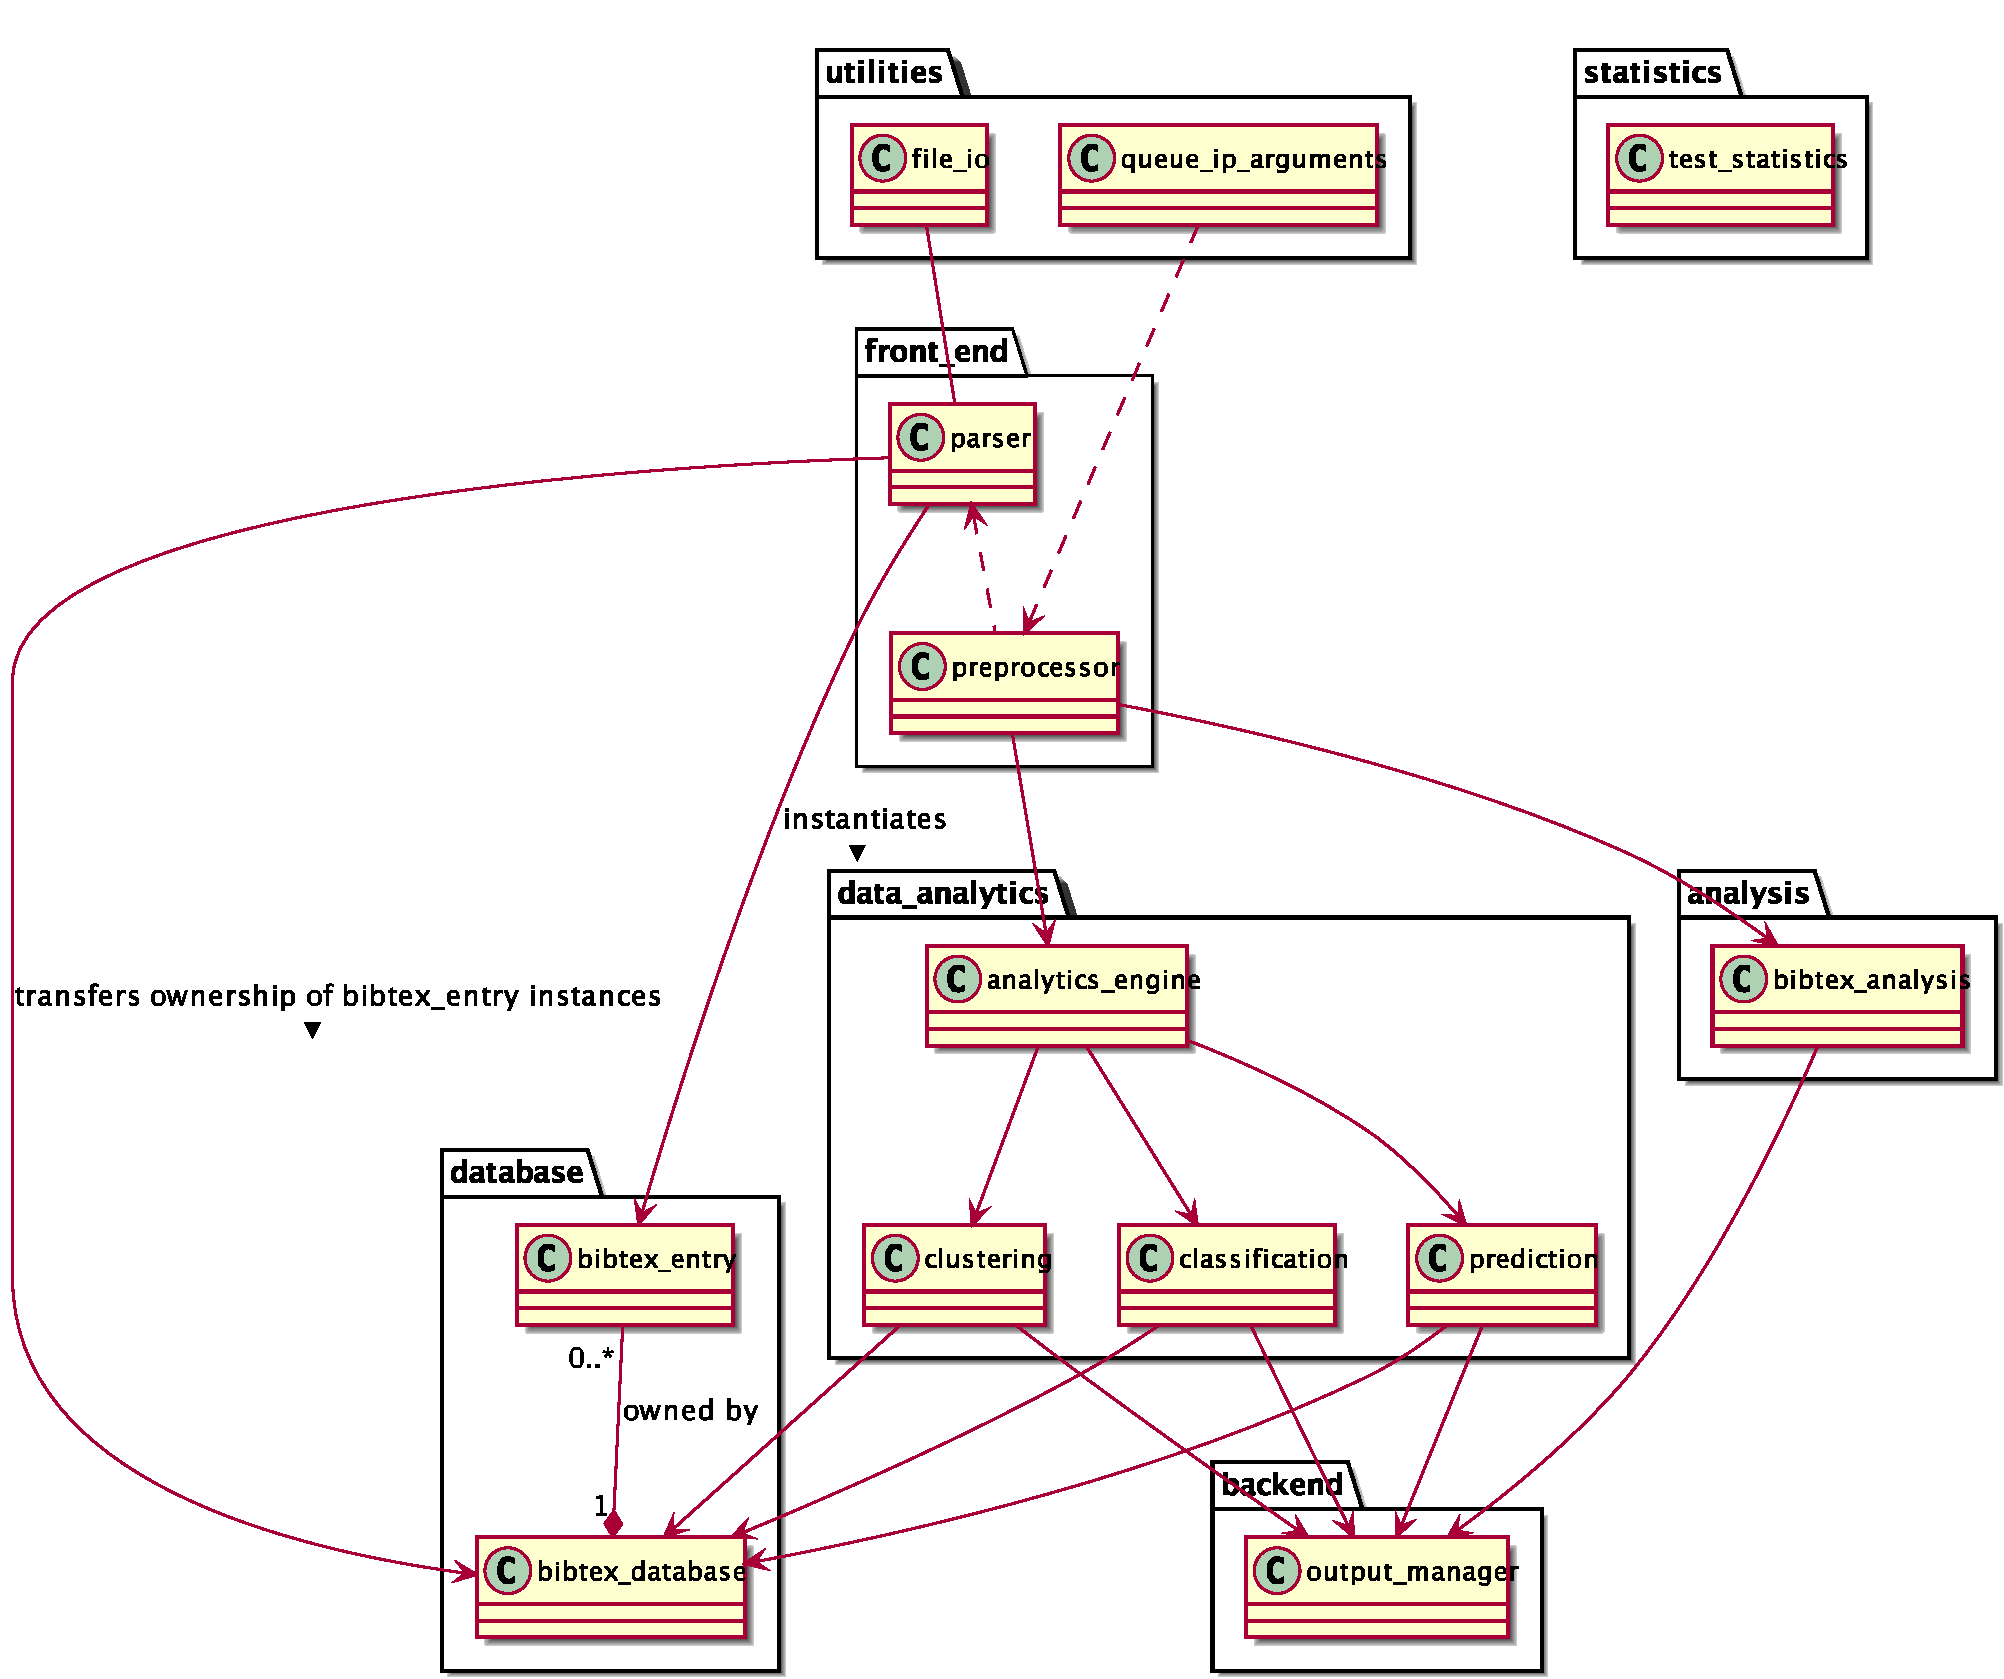
\includegraphics[height=4in]{pics/sw-arch/sw-arch}
\caption{Software architecture of the {\sc Bib}\TeX\ {\it Analytics} project.}
\label{fig:SoftwareArchitecture}
\end{figure}

The {\tt front\_end} package performs the following operations: interacts with the {\tt utilities} package to process command-line input arguments from the user and parse a {\sc Bib}\TeX\ file, instantiates a {\tt bibtex\_database} object to contain instances of {\tt bibtex\_entry} objects, instantiates a {\tt bibtex\_entry} object for each {\sc Bib}\TeX\ entry in the {\sc Bib}\TeX\ file, and passes {\tt bibtex\_entry} objects to the {\tt bibtex\_database} object for storage. Hence, this package also interacts with the {\tt database} package. Using input from the command-line input arguments, it either calls static methods of classes in the {\tt data\_analytics} package or the {\tt analysis} package. \\

When objects in the {\tt data\_analytics} package or the {\tt analysis} package performs operations specified by the command-line input arguments, it interacts with the {\tt bibtex\_database} object in the {\tt database} package to access required information to perform the aforementioned operations. When these operations are completed, objects from either of these packages, {\tt data\_analytics} or {\tt analysis}, pass the computation results to the {\tt output\_manager} in the {\tt backend} package. The {\tt output\_manager} either prints the computation results to a text file in the current working directory or to standard output for display on the {\it Terminal} application. \\

In the {\tt utilities} package, the {\tt queue\_ip\_argument} class has static methods to process command-line input arguments from the user. Likewise, the {\tt file\_io} class has static methods to process an input {\sc Bib}\TeX\ file, which is specified by the user in the command line. \\

Regarding the {\tt data\_analytics} package, the {\tt analytics\_engine} class manages the operations in data analytics, and calls the appropriate machine learning tool. The machine learning tools are: {\tt clustering}, {\tt classification}, and {\tt prediction} (for predictive analytics). \\

Lastly, Figure \ref{fig:SoftwareArchitectureWithHigherCoupling} shows the software architecture of the {\sc Bib}\TeX\ {\it Analytics} project that includes the highly coupled {\tt test\_statistics} class. The {\tt test\_statistics} class collects data from running software test suites during automated regression testing, performs simple statistical analysis on the test data, and reports the result to the user.











\begin{figure}[h]
\centering 
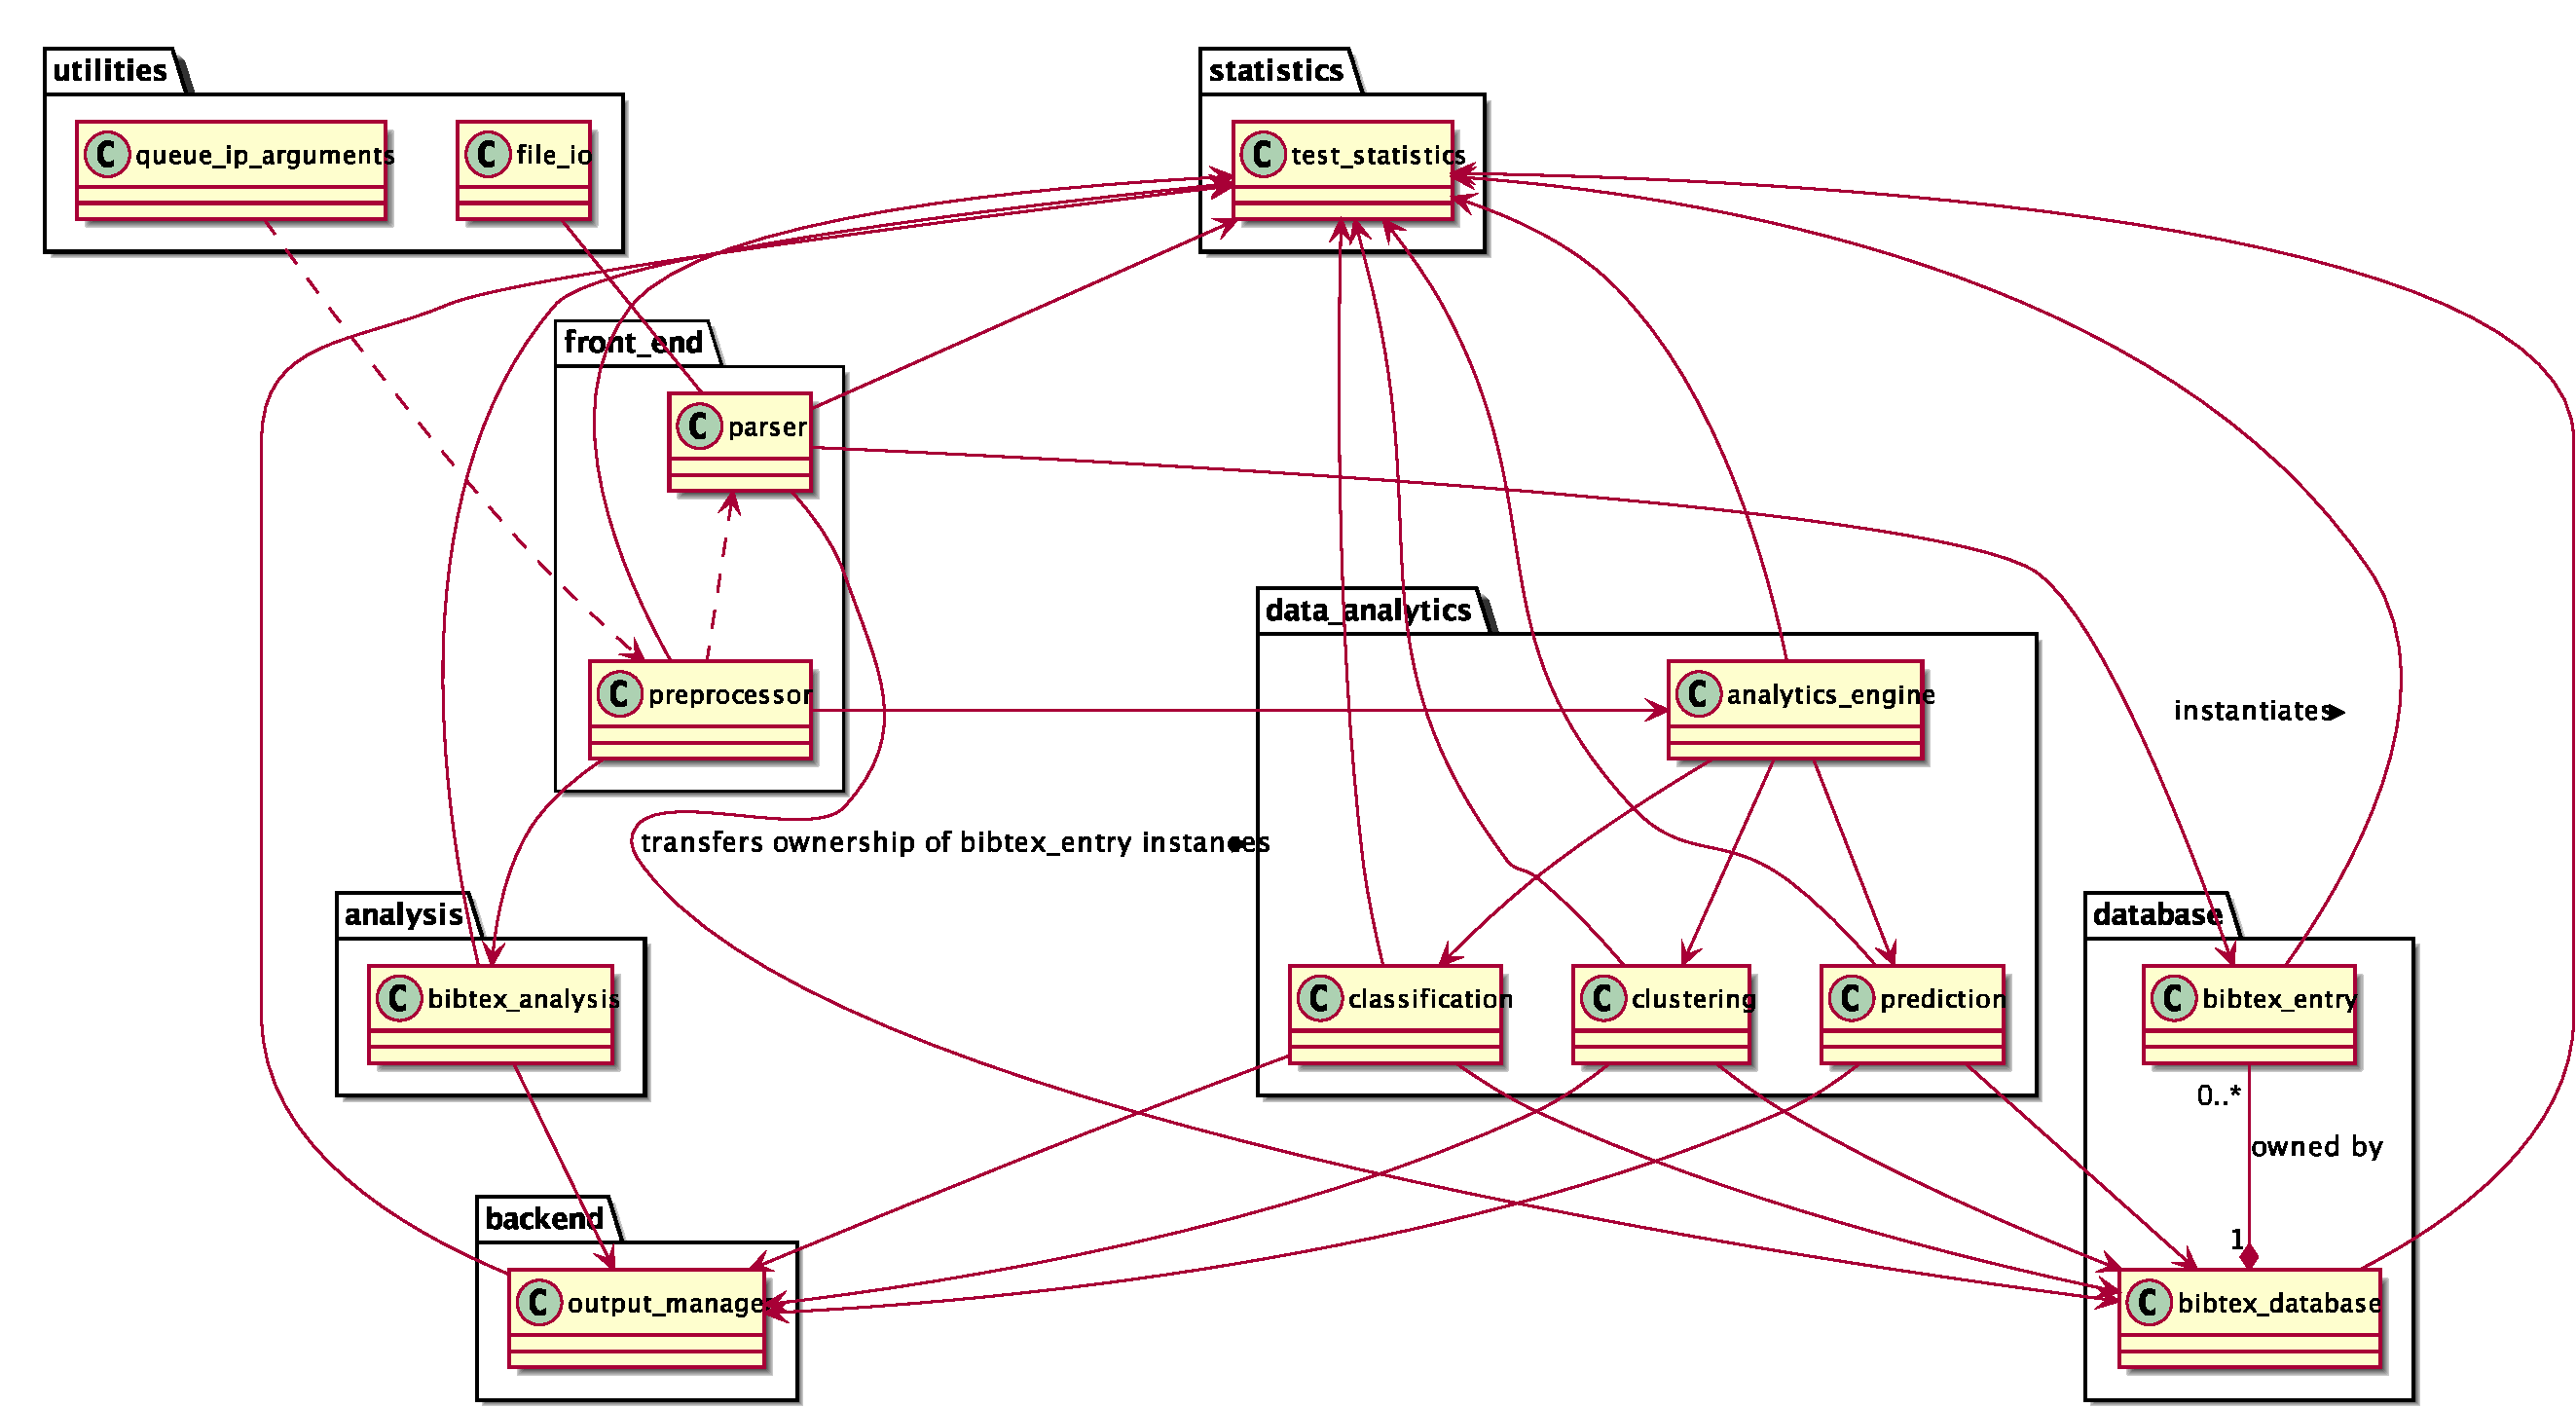
\includegraphics[height=3.5in]{pics/sw-arch-higher-coupling/sw-arch}
\caption{Software architecture of the {\sc Bib}\TeX\ {\it Analytics} project, with highly coupled {\tt test\_statistics} class.}
\label{fig:SoftwareArchitectureWithHigherCoupling}
\end{figure}


















































%%%%%%%%%%%%%%%%%%%%%%%%%%%%%%%%%%%%%%%%%
%	Future Work
%	This is written by Zhiyang Ong as a template for typesetting in LaTeX.

%	The MIT License (MIT)

%	Copyright (c) <2014> <Zhiyang Ong>

%	Permission is hereby granted, free of charge, to any person obtaining a copy of this software and associated documentation files (the "Software"), to deal in the Software without restriction, including without limitation the rights to use, copy, modify, merge, publish, distribute, sublicense, and/or sell copies of the Software, and to permit persons to whom the Software is furnished to do so, subject to the following conditions:

%	The above copyright notice and this permission notice shall be included in all copies or substantial portions of the Software.

%	THE SOFTWARE IS PROVIDED "AS IS", WITHOUT WARRANTY OF ANY KIND, EXPRESS OR IMPLIED, INCLUDING BUT NOT LIMITED TO THE WARRANTIES OF MERCHANTABILITY, FITNESS FOR A PARTICULAR PURPOSE AND NONINFRINGEMENT. IN NO EVENT SHALL THE AUTHORS OR COPYRIGHT HOLDERS BE LIABLE FOR ANY CLAIM, DAMAGES OR OTHER LIABILITY, WHETHER IN AN ACTION OF CONTRACT, TORT OR OTHERWISE, ARISING FROM, OUT OF OR IN CONNECTION WITH THE SOFTWARE OR THE USE OR OTHER DEALINGS IN THE SOFTWARE.

%	Email address: echo "cukj -wb- 23wU4X5M589 TROJANS cqkH wiuz2y 0f Mw Stanford" | awk '{ sub("23wU4X5M589","F.d_c_b. ") sub("Stanford","d0mA1n"); print $5, $2, $8; for (i=1; i<=1; i++) print "6\b"; print $9, $7, $6 }' | sed y/kqcbuHwM62z/gnotrzadqmC/ | tr 'q' ' ' | tr -d [:cntrl:] | tr -d 'ir' | tr y "\n"

%%%%%%%%%%%%%%%%%%%%%%%%%%%%%%%%%%%%%%%%%%%%%%



%%%%%%%%%%%%%%%%%%%%%%%%%%%%%%%%%%%%%%%%%%%
\chapter{Future Work}
\label{chp:FutureWork}

Future work of the {\sc Bib}\TeX\ {\it Analytics} project is described as follows: \vspace{-0.3cm}
\begin{enumerate} \itemsep -4pt
\item Clustering of keywords/keyphrases: \vspace{-0.3cm}
	\begin{enumerate} \itemsep -2pt
	\item {\bf Problem statements}: \vspace{-0.2cm}
		\begin{enumerate} \itemsep -2pt
		\item For an author, find clusters of keyphrases, publishers, journal titles, conferences, \dots
		\item For each keyphrase, determine the cluster of publishers, years, journal titles, conferences, \dots
		\end{enumerate}
	\item Build dictionary of {\it (keyphrase, frequency)} two-tuples (or pairs).
	\item Sort the dictionary based on the frequency term/element, {\it frequency}, in these two-tuples.
	\item Alternate solution: \vspace{-0.2cm}
		\begin{enumerate} \itemsep -2pt
		\item Build a set of {\it (keyphrase, [list of years])} lists.
		\item {\it [list of years]} is a list of years of publications; or it is a set of years for publications that include the keyphrase {\it keyphrase} in its set of keyphrases.
		\item Sort the set based on length of the list of years, {\it [list of years]}.
		\end{enumerate}
	\item If possible, visualize the data for this.
	\item Alternate solution: \vspace{-0.2cm}
		\begin{enumerate} \itemsep -2pt
		\item For each {\sc Bib}\TeX\ entry, there exists a set/cluster of keyphrases.
		\item Find overlaps/intersections between these sets.
		\item E.g., for each set of keyphrases (associated with a publication) with at least three (i.e., more than two) terms, build a list of non-empty overlaps.
		\item Find the largest intersecting subset among the non-disjoint sets. Or, find the top 5-10 most common overlaps.
		\item Refer to books on data visualization for information on visualizing this.
		\item Also, refer to this technical report from Stanford, ``Union-member algorithms for non-disjoint sets.'' See \url{https://dl.acm.org/citation.cfm?id=892212}.
		\end{enumerate}
	\item Compare problem with common subexpression elimination in compiler design, and maximum clique covering problem,
	\item The more common/frequent the subsets are, the hotter the subsets are.
	\item Therefore, find the most frequent intersection. And/or, the greatest intersection.
	\item Problem restated: For each keyphrase, find the largest intersection it has with all the other sets containing the keyword.
	\item That is, capture the largest intersection(s) and map it(/them). This is because multiple sets of the same size could exists. Note that the $2^{\rm nd}/3^{\rm rd}$ largest intersections includes the largest intersection(s) minus 1 (or 2) term(s).
	\item Find overlaps/intersections between these overlaps/intersections.
	\end{enumerate}
\item Classification: \vspace{-0.3cm}
	\begin{enumerate} \itemsep -2pt
	\item Classify each keyphrase/topic into hot or not.
	\item Classify each author into hot or not.
	\item Note that since the size of my {\sc Bib}\TeX\ database is small, but significant, compared to reality, put these results of classification into proper perspective.
	\end{enumerate}
\item Predictive analytics: \vspace{-0.3cm}
	\begin{enumerate} \itemsep -2pt
	\item Recognize trends, predict trends.
	\item For the last 5 (or 8) years, find the (emerging) trends of hot topics.
	\end{enumerate}
\item For a given keyphrase, provide a list of {\sc Bib}\TeX\ entries that contain that keyphrase in their keyword {\sc Bib}\TeX\ field.
\item Perform miscellaneous tasks to clean up the {\sc Bib}\TeX\ file.
\item Check if the ampersand is surrounded by curly braces and set to the normal (non-Italics) font.
\item For each conference proceedings, check if its abbreviation is placed within round brackets after the title of the conference proceedings. Also, Check if there is no comma between the title and the abbreviation.
\item Write a script to extract the keywords from the {\sc Bib}\TeX\ repository, arrange them in alphabetical order, and pipe them to an output file.
\item Check if the addresses of the publications have the U.S. states in capital letters.: \vspace{-0.3cm}
	\begin{enumerate} \itemsep -2pt
	\item If I use abbreviations for states and territories in Australia and Canada, do likewise.
	\item For publications outside the U.S., (and Australia and Canada), ignore this.
	\end{enumerate}
\item Check if DOIs and/or URL fields are missing, if the following fields (metadata for {\it BibDesk}) exists: \vspace{-0.3cm}
	\begin{enumerate} \itemsep -2pt
	\item Bdsk-Url-1
	\end{enumerate}
\item Additional tasks: \vspace{-0.3cm}
	\begin{enumerate} \itemsep -2pt
	\item {\tt extract\_citations.py}: \vspace{-0.2cm}
		\begin{enumerate} \itemsep -2pt
		\item Run as: {\it ./extract\_citations.py [LaTeX sources] [BibTeX output]}
		\item Produces an intermediate output, which is a set of {\sc Bib}\TeX\ keys that uniquely identifies a matching {\sc Bib}\TeX\ entry in my {\sc Bib}\TeX\ database.
		\end{enumerate}
	\item {\tt not\_defined\_references.py}: \vspace{-0.2cm}
		\begin{enumerate} \itemsep -2pt
		\item Run as: {\bf ./not\_defined\_references.py  [LaTeX sources] [BibTeX input]}
		\item Check if this citation uses a undefined reference
		\item No output required.
		\end{enumerate}
	\item {\tt uncomment\_latex\_src\_files.py}: \vspace{-0.2cm}
		\begin{enumerate} \itemsep -2pt
		\item Run as: {\bf ./uncomment\_latex\_src\_files.py [dirty LaTeX source files] [clean LaTeX source files]}
		\item Remove comments from \LaTeX\ source files. Non importante.
		\end{enumerate}
	\end{enumerate}
\item Find emerging research trends to consider pivoting towards, or to get involved in side projects \vspace{-0.3cm}
	\begin{enumerate} \itemsep -2pt
	\item E.g., benchmark adiabatic quantum computers with topological computers and universal quantum computers \cite{Tandon2017}.
	\end{enumerate}
\end{enumerate}
































%%%%%%%%%%%%%%%%%%%%%%%%%%%%%%%%%%%%%%%%%%%%%
%%%%%%%%%%%%%%%%%%%%%%%%%%%%%%%%%%%%%%%%%%%%%
%
%	End of document
%
%	Inserting references
%
%%%%%%%%%%%%%%%%%%%%%%%%%%%%%%%%%%%%%%%%%%%%%
%%%%%%%%%%%%%%%%%%%%%%%%%%%%%%%%%%%%%%%%%%%%%
%	Beginning of BACK MATTER: bibliography, indexes and colophon
%\backmatter
\appendix

{\linespread{1}
\bibliographystyle{plain}
%\bibliography{~/Documents/ricerca/lassi-bibtex/references}
\bibliography{/Users/zhiyang/Documents/ricerca/lassi-bibtex/references}
\addcontentsline{toc}{chapter}{Bibliography}
}
\end{document}